\section{Exploraci??n Univariada}\label{univariada}




El estudio se hizo para los 32 departamentos de Colombia y mediante este, se determino que nuestro pais ocupa la casilla 91 dentro del listado de 186 paises a los que las Naciones Unidas para el Desarrollo (PNUD) le miden el Indice de Desarrollo Humano (IDH). 
Esto la ubica por debajo de paises como Panama, Peru y Cuba, y representa una perdida de cuatro puestos respecto a su ubicacion en el estudio del 2012.  
En el documento "El Ascenso del Sur: Progreso Humano en un Mundo Diverso", del PNUD, se muestran algunos avances en materia de educacion en toda Latinoamerica, pero Colombia sigue teniendo ciertos inconvenientes en este sentido.  
El estudio revela que los ni??os en Colombia estudian en promedio 7,3 a??os mientras el "periodo esperado de escolaridad" son 13,6. 

% Table created by stargazer v.5.2.2 by Marek Hlavac, Harvard University. E-mail: hlavac at fas.harvard.edu
<<<<<<< HEAD
% Date and time: Fri, Jun 29, 2018 - 17:21:36
=======
% Date and time: vie., jun. 29, 2018 - 5:09:48 p. m.
>>>>>>> 89dcf29e5b31ddb0d151fffe93ffa6d59bf5d5ad
\begin{table}[!htbp] \centering 
  \caption{Medidas estad??sticas} 
  \label{stats} 
\begin{tabular}{@{\extracolsep{5pt}}lccccc} 
\\[-1.8ex]\hline 
\hline \\[-1.8ex] 
Statistic & \multicolumn{1}{c}{Mean} & \multicolumn{1}{c}{Median} & \multicolumn{1}{c}{St. Dev.} & \multicolumn{1}{c}{Min} & \multicolumn{1}{c}{Max} \\ 
\hline \\[-1.8ex] 
IDH & 0.802 & 0.804 & 0.042 & 0.691 & 0.879 \\ 
Poblacion.Cabecera & 1,196,730.000 & 717,197 & 1,982,287.000 & 13,090 & 10,070,801 \\ 
Poblacion.Resto & 360,590.300 & 268,111.5 & 331,887.600 & 21,926 & 1,428,858 \\ 
Poblacion.Total & 1,557,320.000 & 1,028,429 & 2,202,522.000 & 43,446 & 10,985,285 \\ 
\hline \\[-1.8ex] 
\end{tabular} 
\end{table} \centering


\begin{figure}[h]
\centering
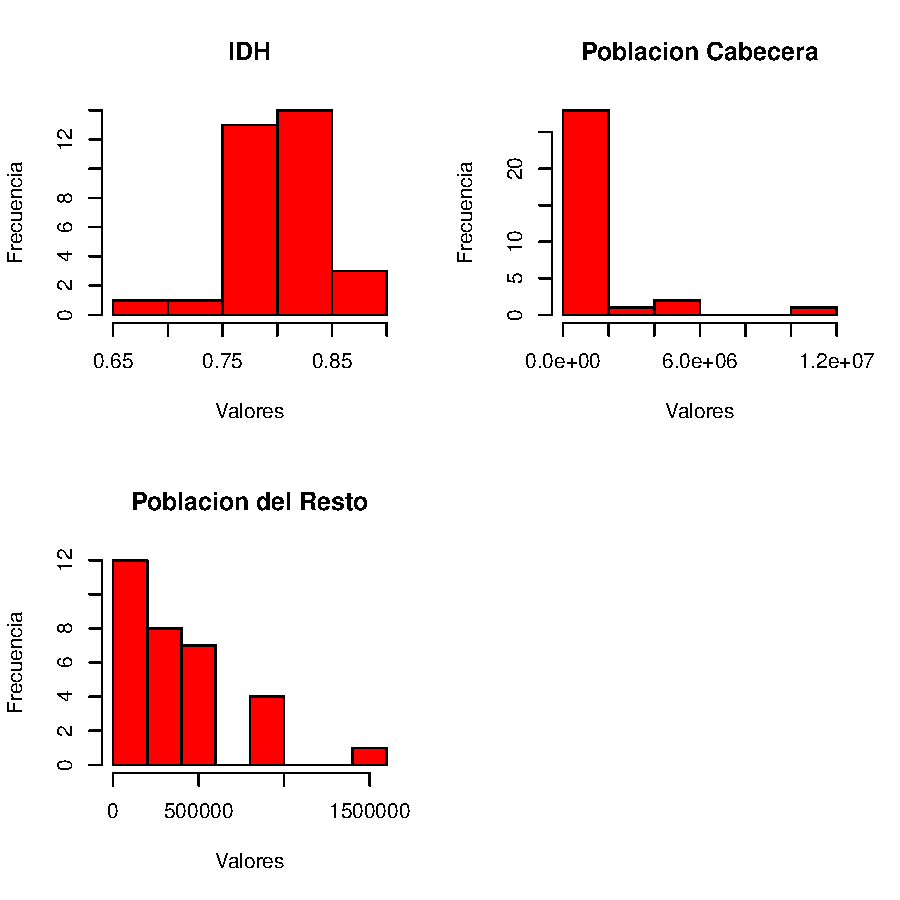
\includegraphics{univariada-hist}
\caption{Distribuci?n de Indicadores}
\label{hist}
\end{figure}

Si quieren normalizar dado el sesgo de las poblaciones, se tranforma con logaritmo en case 10 y quedaria asi:

\begin{figure}[h]
\centering
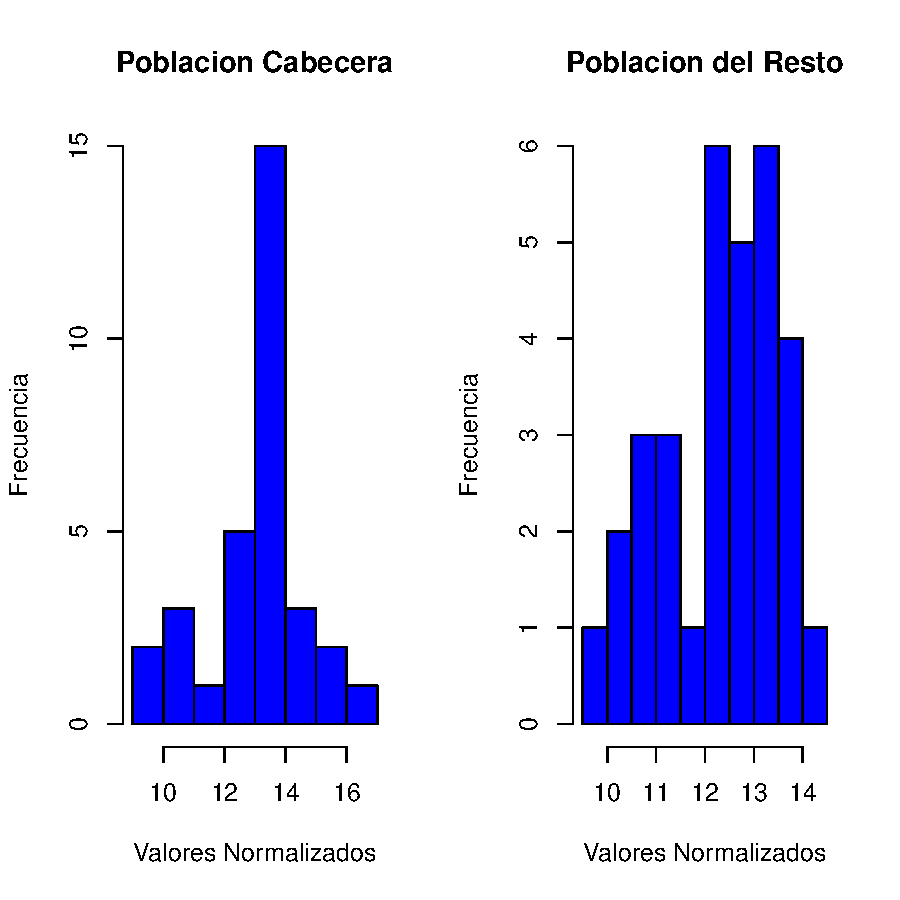
\includegraphics{univariada-hist1}
\caption{Distribuci?n de Indicadores de Poblaciones Normalizado}
\label{hist1}
\end{figure}

\endinput
